\subsection{Fuel salt reprocessing system}

\begin{frame}
  \frametitle{Fuel salt reprocessing system overview: gas separation}
  Gaseous fission products (e.g., Xe, Kr) must be removed from the fuel salt 
  to avoid reactor
poisoning. 
  
      \begin{columns}
      	\column[t]{4.5cm}
    \begin{block}{Noble gases removal process:}
      \begin{enumerate}
      	\item bubble generator injects He bubbles in the salt stream
      	\item noble gases migrate to the He bubbles due to their insolubility 
      	in salt
      	\item gas separator discharges the poison-rich bubbles from the salt
      \end{enumerate}
    \end{block}    	
      	
     	\column[t]{7cm}
  \begin{figure}[t]
	  \centering
	  		\vspace{-8mm}
		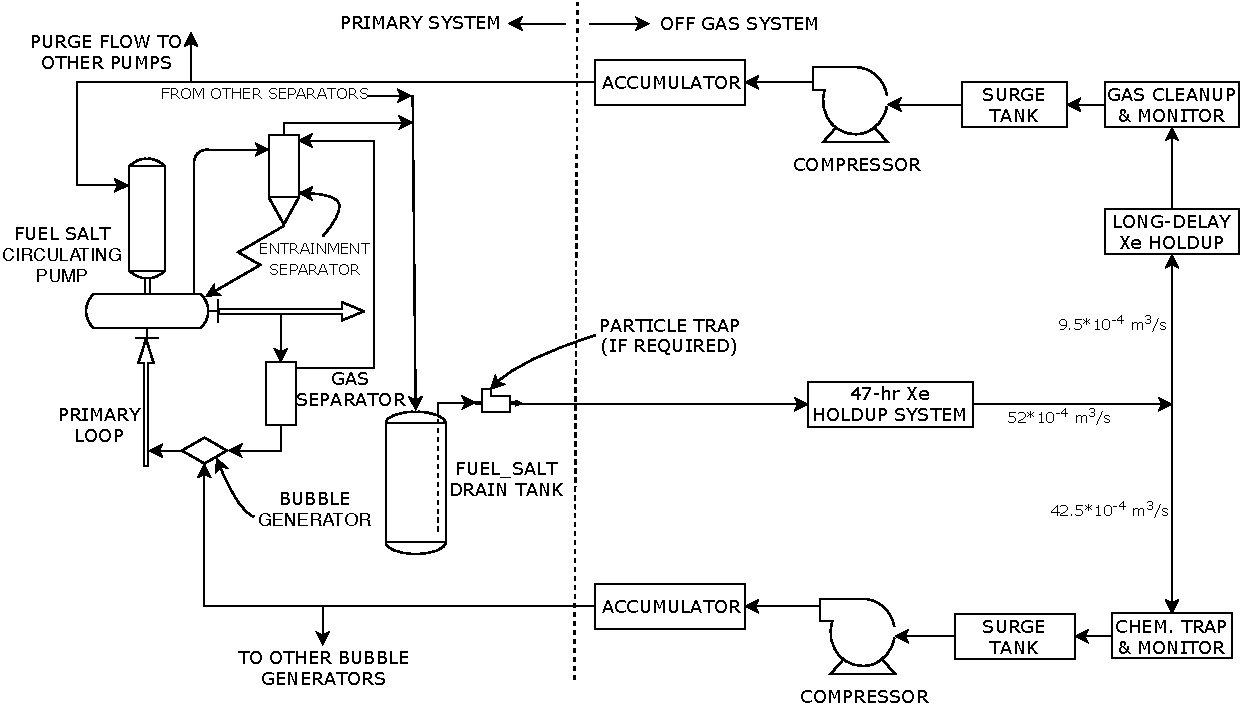
\includegraphics[width=1.03\textwidth]{../figures/gas_separation.pdf}
	\caption{Schematic flow diagram of the \gls{MSBR} gas separation system 
	(figure reproduced from Robertson \emph{et al.}  
	\cite{robertson_conceptual_1971}).} 
    \end{figure}

	\end{columns}
\end{frame}

\begin{frame}
  \frametitle{Mathematical model for gas separation efficiency}
  		\vspace{-3mm}
  \begin{figure}[t]
   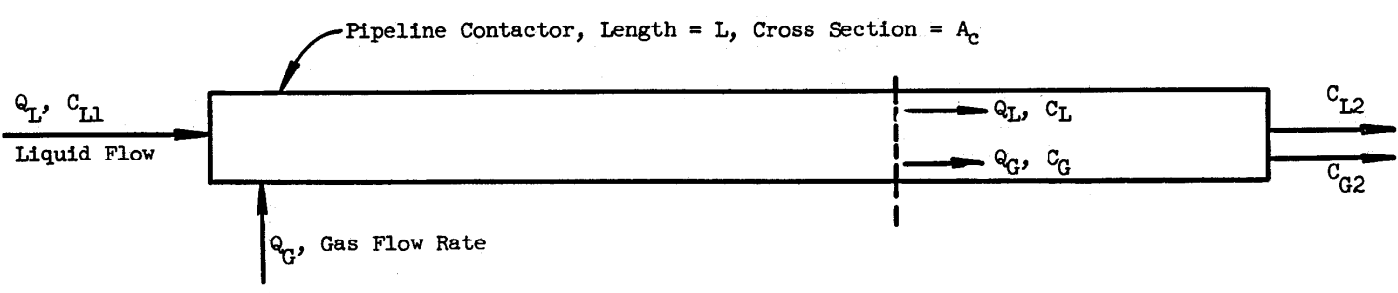
\includegraphics[width=0.7\textwidth]{./images/pipeline_contactor.png}
   		\vspace{-2mm}
   \caption{Flow diagram for gas separator (figure reproduced from Peebles 
   \emph{et al.} \cite{peebles_removal_1968}).}
    \end{figure}
		\vspace{-2mm}
Xenon removal efficiency ($\epsilon_{Xe}$) in a gas separation system  
\cite{peebles_removal_1968}:
\begin{align}
& \qquad\qquad \epsilon_{Xe} = \frac{1-e^{-\beta}}{1+\alpha} \nonumber \\
\alpha &= \frac{RTQ_{L}}{HQ_{G}} \nonumber \\
\beta &= \frac{K_L a A_C L (1+\alpha)}{Q_{L}} \nonumber \\
Q_{L}&= \mbox{volumetric salt flow rate} \nonumber \\
Q_{G}&= \mbox{volumetric helium flow rate} \nonumber \\
H &= \mbox{Henry's law constant} \nonumber \\
a &= \mbox{gas-liquid interfacial area} \nonumber \\
K_L &= \mbox{liquid phase mass transfer coefficient.} \nonumber
\end{align}

\end{frame}

\begin{frame}
\frametitle{Fuel chemical processing system overview: rare earths and 
Pa removal}
	\begin{figure}[htp!] % replace 't' with 'b' to 
		\centering
			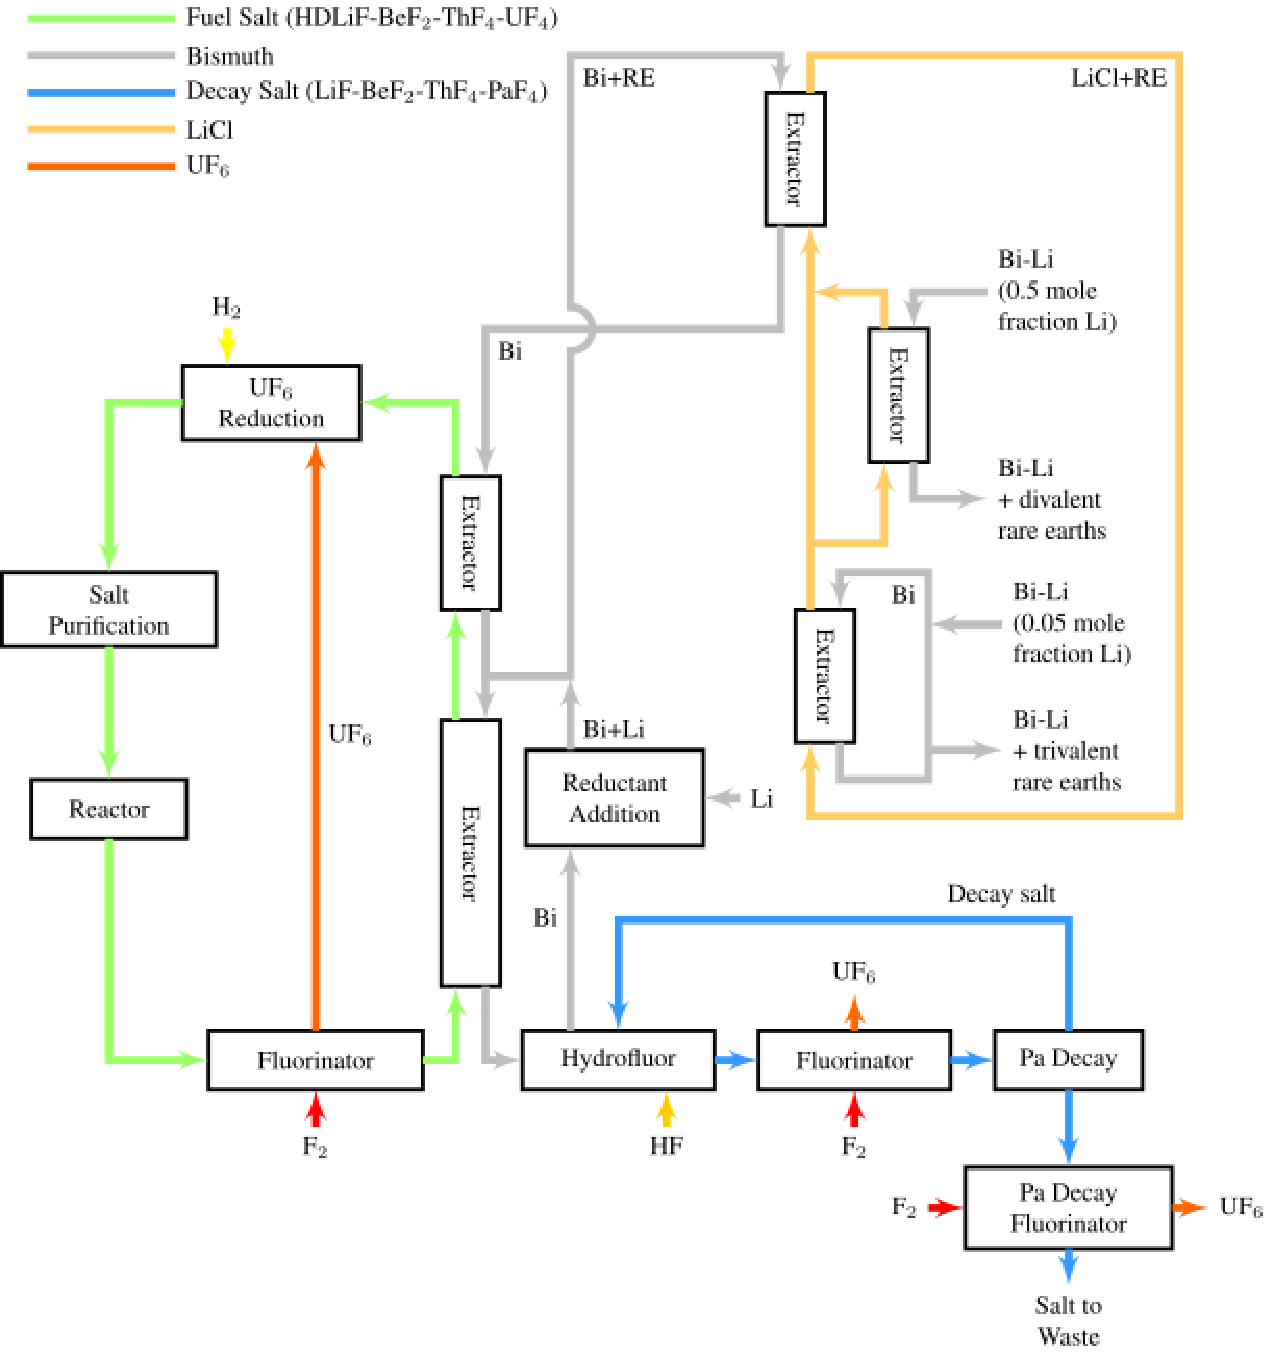
\includegraphics[width=0.57\textwidth]{../figures/flowsheet.pdf}
			\vspace{-2mm}
		\caption{Diagram of chemical processing scheme for \gls{MSBR} 
		(reproduced from Sorensen \cite{sorensen_one-fluid_2006}).} 
	\end{figure}
	
\end{frame}
